\documentclass[oneside]{book}

% 汉语支持
% 这里没有使用ctexbook的原因是因为其会造成在TeXstudio编辑时对\chapter命令
% 的提示不正常,并进而造成在TeXstudio界面左侧的Structure显示不正常。
\usepackage[fontset=ubuntu]{ctex}
\usepackage{geometry}% 用于页面设置
\usepackage[dvipsnames, svgnames, x11names]{xcolor}% 颜色支持
\usepackage{graphicx}% 图形支持
\usepackage[
  colorlinks=true,
  linkcolor=Navy,
  urlcolor=Navy,
  citecolor=Navy,
  anchorcolor=Navy
]{hyperref}% 设置超链接颜色
\usepackage{enumerate}% 枚举支持
\usepackage{minted}% 代码高亮支持

% 设置显示风格。风格名称可以用“pygmentize -L styles”查看
\usemintedstyle{xcode}

% 纸张设置
\geometry{
  a4paper,
  left = 1in,
  right = 1in,
  top = 1in,
  bottom = 1in
}

\emergencystretch = \maxdimen% 断字处理
\setlength{\parindent}{2em}% 缩进
\setlength{\parskip}{1ex} % 段间距

% 把篇章名称part、chapter换成中文
\usepackage{titlesec}% 可使用\usepackage[center]{titlesec}设置对齐方式
\titleformat{\part}{\centering\Huge\bfseries}{第\,\thepart\,篇}{0em}{\\}
\titleformat{\chapter}{\raggedright\Huge\bfseries}{第\,\thechapter\,章}{1em}{}

% ------------------ 开始 -------------------
\begin{document}


  % ------------------ 封面 -------------------
  \begin{titlepage}%
    \begin{center}
      
\includegraphics[width=.3\textwidth]{images/cover.png}

      \vspace{2ex}

      \Huge\textbf{Sunflower项目记录}\normalsize

      \vspace{8ex}

      编写:陆巍




    \vfill

    2023年12月29日
    \end{center}

  \end{titlepage}


  % ------------------ 前言 -------------------
  \frontmatter% 关闭章节序号,页码使用罗马数字


  \chapter{前言}


  % ------------------ 目录 -------------------
  \tableofcontents% 生成目录


  % ------------------ 正文 -------------------
  \mainmatter

  \chapter{概述}
Sunflower项目是一个小型网站项目,其内容包括网站和一个小型的Web Server。


\chapter{需求分析}


\section{开发平台和技术}
\begin{itemize}
  \item 项目在 Ubuntu 22.04 操作系统上开发。
  \item 开发使用的编程语言包括 HTML、CSS、JavaScript 和 Go 语言。
  \item 数据库选用 PostgreSQL 14.10。
  \item Web 框架选用 Gin。
\end{itemize}


\section{网站布局}
左右分栏结构,左栏小、右栏大。


\section{设计特点}
临时标志如下:
\begin{center}
  
\includegraphics[width=.3\textwidth]{images/logo.png}
\end{center}


\section{所需的特点和功能}


\subsection{第一阶段目标}
初步目标是建立一个任务管理系统,功能需要如下:
\begin{enumerate}
  \item 可展示任务总体和按状态、类别分组的列表;
  \item 能够新增、修改和删除任务类别;
  \item 能够新增、修改和删除任务;
  \item 表现任务依赖关系;
  \item 可显示任务的时间安排;
\end{enumerate}


\section{内容和照片的空间分布}


\subsection{布局}
\begin{center}
  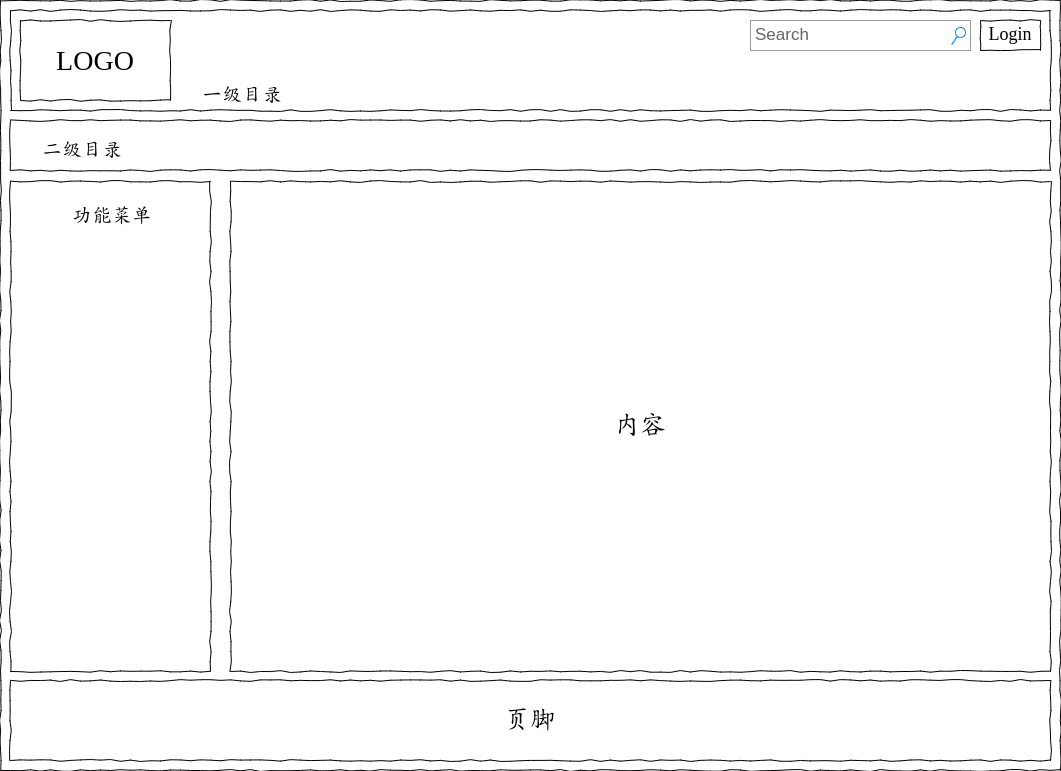
\includegraphics[width=\textwidth]{images/页面布局.png}
\end{center}


\section{页眉和页脚细节}


\section{联系表单和订阅详情}

\end{document}
